\documentclass{beamer}
\usepackage{graphicx}
\graphicspath{{./img/}}

\AtBeginSection[]{
    \begin{frame}{Table of Contents}
        \tableofcontents[currentsection]
    \end{frame}
}

%%%%%%%%%%%%%%%%%%%%%%% DIY 1: Complete, compile %%%%%%%%%%%%%%%%%%%%%%%
\title{Very Pretty Beamer}
\author{Your Name}
\institute{JI}
\date{2023}

\begin{document}
\frame{\titlepage}

%%%%%%%%%%%%%%%%%%%%%%%%%% DIY 2: Multicolumn %%%%%%%%%%%%%%%%%%%%%%%%%%
\begin{frame}{$\Box\Box\Box\Box,\Box\Box\langle\langle\Box\Box\rangle\rangle$}
    You are right, but \LaTeX\ is a brand-new typesetting system
    independently developed by Leslie Lamport. The system is based
    on a language called ``\TeX'', which powers ``macro packages'',
    to guide your writing. You will be the powerful role known as
    the ``user'', reading documentation and using all kinds of
    commands and environments; you will write impressive articles
    and beamers — and in the meantime reveal the truth of ``\LaTeX''.

    % divide columns here

    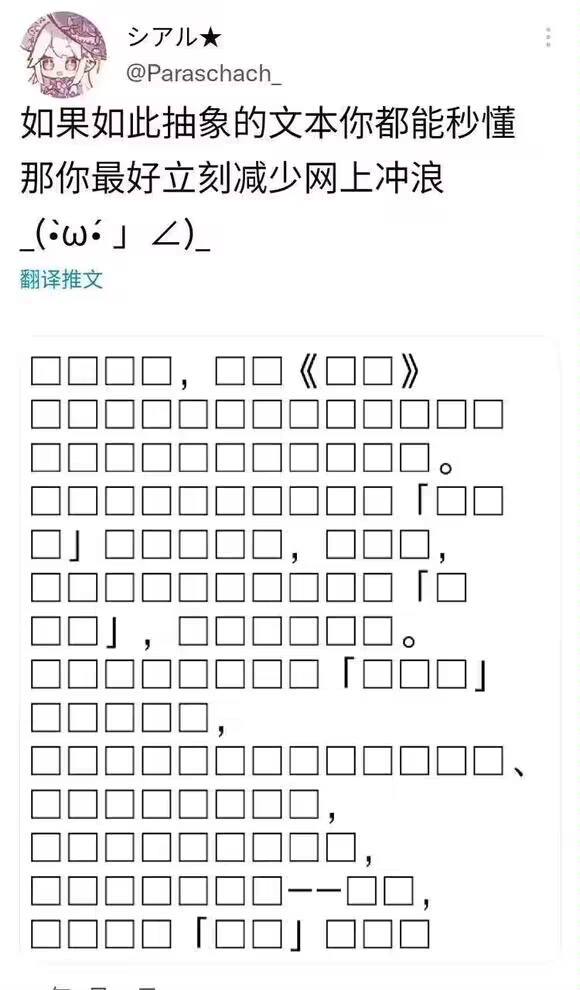
\includegraphics[width=\textwidth]{genshin}
\end{frame}

%%%%%%%%%%%%%%%%%%%%%%%%%%% DIY 3: Sections %%%%%%%%%%%%%%%%%%%%%%%%%%%%
\begin{frame}{Results and Measurements}
\end{frame}
\begin{frame}{Resonance Method}
\end{frame}
\begin{frame}{Phase Difference Method}
\end{frame}

\begin{frame}{Uncertainty analysis}
\end{frame}
\begin{frame}{Resonance Method}
\end{frame}
\begin{frame}{Phase Difference Method}
\end{frame}

\begin{frame}{Conclusions}
\end{frame}

%%%%%%%%%%%%%%%%%%%%%%%%%%% DIY 4: Blocks %%%%%%%%%%%%%%%%%%%%%%%%%%%%%%
\begin{frame}{Blocks}
    \[
        e^{i \theta} = \cos \theta + i \sin \theta
    \]

    \[
        e^{i \theta + \varphi} = e^\varphi (\cos \theta + i \sin \theta)
    \]

    \[
        e^{i \pi} = -1
    \]

    In physics, the convention is $j$ because $i$ stands for current.
\end{frame}

%%%%%%%%%%%%%%%%%%%%%%%%%% DIY 5: Overlays %%%%%%%%%%%%%%%%%%%%%%%%%%%%%
\begin{frame}{Overlays}
% Make this paragraph the only thing on the first slide
Here at JI, we go international!

So let's say hello to the whole world: China, US, France, Germany,
Korea, Japan…

% Make items appear one by one in reverse order
\begin{itemize}
    \item \rotatebox[origin=c]{180}{in Australia!}
    \item \rotatebox[origin=c]{180}{warmest greetings to our friends}
    \item \rotatebox[origin=c]{180}{And we won't forget to send}
\end{itemize}
\end{frame}
\end{document}
